% This file was created by tikzplotlib v0.8.5.
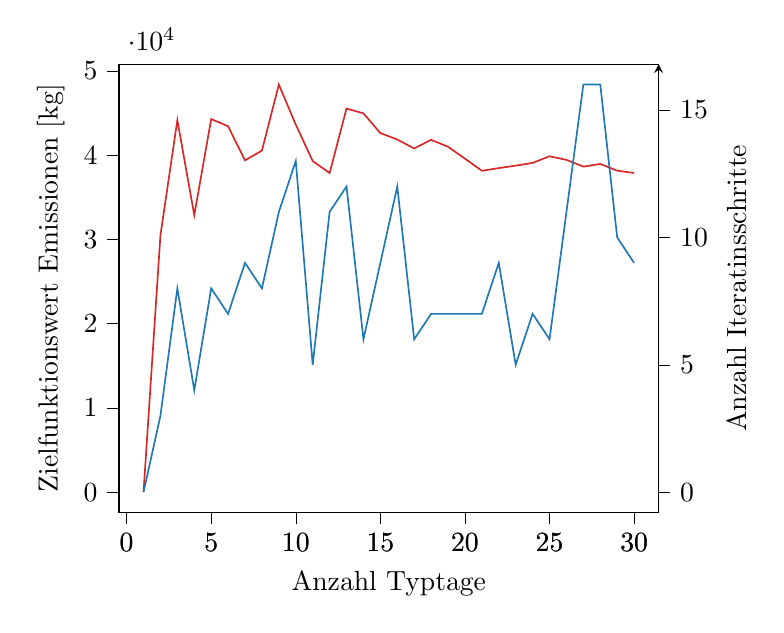
\begin{tikzpicture}

\definecolor{color0}{rgb}{0.83921568627451,0.152941176470588,0.156862745098039}
\definecolor{color1}{rgb}{0.12156862745098,0.466666666666667,0.705882352941177}

\begin{axis}[
tick align=outside,
tick pos=left,
x grid style={white!69.01960784313725!black},
xlabel={Anzahl Typtage},
xmin=-0.45, xmax=31.45,
xtick style={color=black},
y grid style={white!69.01960784313725!black},
ylabel={Zielfunktionswert Emissionen [kg]},
ymin=-2418.836, ymax=50795.556,
ytick style={color=black}
]
\addplot [semithick, color0]
table {%
1 0
2 30494.82
3 44160.41
4 32878.5
5 44286.04
6 43425.25
7 39380.14
8 40541.8
9 48376.72
10 43620.3
11 39303.31
12 37877.01
13 45533.13
14 44957.85
15 42621.35
16 41855.97
17 40790.18
18 41821.16
19 40997.61
20 39587.41
21 38143.49
22 38465.22
23 38753.05
24 39077.35
25 39865.98
26 39439.68
27 38636.08
28 38951.84
29 38161.65
30 37877.62
};
\end{axis}

\begin{axis}[
axis y line=right,
tick align=outside,
x grid style={white!69.01960784313725!black},
xmin=-0.45, xmax=31.45,
xtick pos=left,
xtick style={color=black},
y grid style={white!69.01960784313725!black},
ylabel={Anzahl Iteratinsschritte},
ymin=-0.8, ymax=16.8,
ytick pos=right,
ytick style={color=black}
]
\addplot [semithick, color1]
table {%
1 0
2 3
3 8
4 4
5 8
6 7
7 9
8 8
9 11
10 13
11 5
12 11
13 12
14 6
15 9
16 12
17 6
18 7
19 7
20 7
21 7
22 9
23 5
24 7
25 6
26 11
27 16
28 16
29 10
30 9
};
\end{axis}

\end{tikzpicture}
